  Dieses Kapitel behandelt die Analyse von Java Swing Applikationen. Die
  Analyse betrifft die Swing Komponenten, und Komponenten die in einen
  Zusammenhang mit Swing Komponenten stehen. Es werden die gezeigten
  Methoden zur Analyse von Java Swing Applikationen aus dem Kapitel 
  \ref{chapter:MethodenZurAnalyseVonJavaSwingApplikationen}
  (\nameref{chapter:MethodenZurAnalyseVonJavaSwingApplikationen}, S.
  \pageref{chapter:MethodenZurAnalyseVonJavaSwingApplikationen}ff) angewendet.
  Als Ergebnis wird eine Kategorisierung der verwendeten Swing Komponenten
  aufgelistet. Der Ablauf wird in der Abbildung
  \ref{img:kompletteApplikationsAnalyse} dargestellt.
  \newline

  
  \section{Auswahl der Java Swing Applikationen}
  
  Es sollen drei Applikationen, welche von der Zürcher Kantonalbank entwickelt
  wurden, analysiert werden. Die Applikationen sollen mit Java Swing entwickelt
  worden sein. Die Applikationen werden in der Tabelle
  \ref{tab:zuAnalysierendeJavaSwingApplikationen} aufgelistet.
  \newline
  
  \begin{table}[ht]
    \sffamily 
    \begin{center}
      \begin{tabular}{llp{2cm}p{3.5cm}}
        \toprule
        \textbf{Applikation} & \textbf{Version} & \textbf{Sourcecode vorhanden}
        & \textbf{GUI enthält sensible Informationen}\\
        \midrule
        Strukti Live & 1.2 & Ja & Nein\\
        Strukti Online & 2.10.0 & Ja & Ja\\
        Hedo Tool & 1.0.710 & Ja & Ja\\
        \bottomrule
      \end{tabular}
      \caption{Zu analysierende Java Swing Applikationen}
      \label{tab:zuAnalysierendeJavaSwingApplikationen}
    \end{center}
  \end{table}
  
  \section{Begründung}
  
  \begin{description}
  \item[Strukti Live]
  Wurde gewählt, weil diese Applikation von der ZKB veröffentlicht wurde. Somit
  werden bei der Analayse keine sensiblen Informationen preisgegeben.
  
  \item[Strukti Online]
  Wurde gewählt, weil eine mögliche Migration zur Web Applikation schon einmal
  in der \ac{ZKB} zur Diskussion stand.
  
  \item[Hedo Tool]
  Wurde gewählt, da die Applikation über ein hochstehendes \ac{GUI} verfügt.
  \end{description}
  
  \section{Strukti Live}
  
  Strukti Live ist ein Lerntool der Zürcher Kantonalbank für strukturierte
  Produkte. Die Applikation kann auf dem Internetauftritt \footnote{Unter 
  \url{http://www.zkb.ch/struktilive} sind alle nötigen Informationen zu Strukti
  Live enthalten.} der \ac{ZKB} heruntergeladen werden. Es wurde die aktuelle
  Version 1.2 für die Analyse verwendet.
  
  In der Tabelle \ref{tab:bibliothekenStruktiLive} sind alle verwendeten
  Bibliotheken, welche eine Interaktion mit dem \ac{GUI} haben, ersichtlich.
  \newline
  
  \begin{table}[ht]
    \sffamily 
    \begin{center}
      \begin{tabular}{lp{4.5cm}ccp{2cm}}
        \toprule
        \textbf{Bibliothek} & \textbf{Funktion} & \textbf{Version} &
        \textbf{Lizenz} & \textbf{Quellcode vorhanden}\\
        \midrule
        core-renderer.jar & XHtml und CSS Renderer für Swing & R8 & LGPL & Ja\\
        %bogatyr\_0.60.jar & Abstraktion einiger Swing Komponenten & 0.60 & GPL
        %& Ja\\
        jfreechart-1.0.10.jar & Charting Library für Java & 1.0.10 & LGPL & Ja\\
        %jcommon-1.0.13.jar & JFreeChart extension & 1.0.13 & LGPL & Ja\\
        %ZKB\_CICD\_0.40.jar & Swing Komponenten im ZKB Design & 0.40 & - & Ja\\
        \bottomrule
      \end{tabular}
      \caption{Verwendete Bibliotheken von Strukti Live 1.2}
      \label{tab:bibliothekenStruktiLive}
    \end{center}
  \end{table}
  
  \subsection{Gefundene Komponenten}
  
  \subsubsection{Top-Level-Komponenten}
  
  \begin{itemize}
    \item \(javax.swing.JDialog\), siehe Abbildung \ref{img:SL-02}
    \item \(javax.swing.JFrame\), siehe Abbildung \ref{img:SL-01}
  \end{itemize}
  
  \subsubsection{Intermediate-Komponenten}
  
  \begin{itemize}
    \item \(javax.swing.JPanel\), siehe Abbildung \ref{img:SL-01}
    \item \(javax.swing.JRootPane\), siehe Abbildung \ref{img:SL-01}
    \item \(javax.swing.JScrollPane\), siehe Abbildung \ref{img:SL-01}
    \item \(javax.swing.JTabbedPane\), siehe Abbildung \ref{img:SL-03}
  \end{itemize}
  
  \subsubsection{Atomic-Komponenten}
  
  \begin{itemize}
    \item \(javax.swing.JButton\), siehe Abbildung \ref{img:SL-01}
    \item \(javax.swing.JCheckBox\), siehe Abbildung \ref{img:SL-01}
    \item \(javax.swing.JLabel\), siehe Abbildung \ref{img:SL-01}
    \item \(javax.swing.JRadioButton\), siehe Abbildung \ref{img:SL-02}
    \item \(javax.swing.JSlider\), siehe Abbildung \ref{img:SL-02}
    \item \(javax.swing.JTextField\), siehe Abbildung \ref{img:SL-02}
    \item \(javax.swing.JToolTip\), siehe Abbildung \ref{img:SL-03}
  \end{itemize}
  
  \subsubsection{Spezielle Komponenten}
  
  \begin{itemize}
    \item \(javax.swing.JLabel\) als externer Link, siehe Abbildung
    \ref{img:SL-03}
    \item \(org.jfree.chart.JFreeChart\), siehe Abbildung \ref{img:SL-02}
    \item \(org.xhtmlrenderer.simple.XHTMLPanel\), siehe Abbildung
    \ref{img:SL-03}
  \end{itemize}
  
  \begin{figure}[htb]
    \begin{center}
      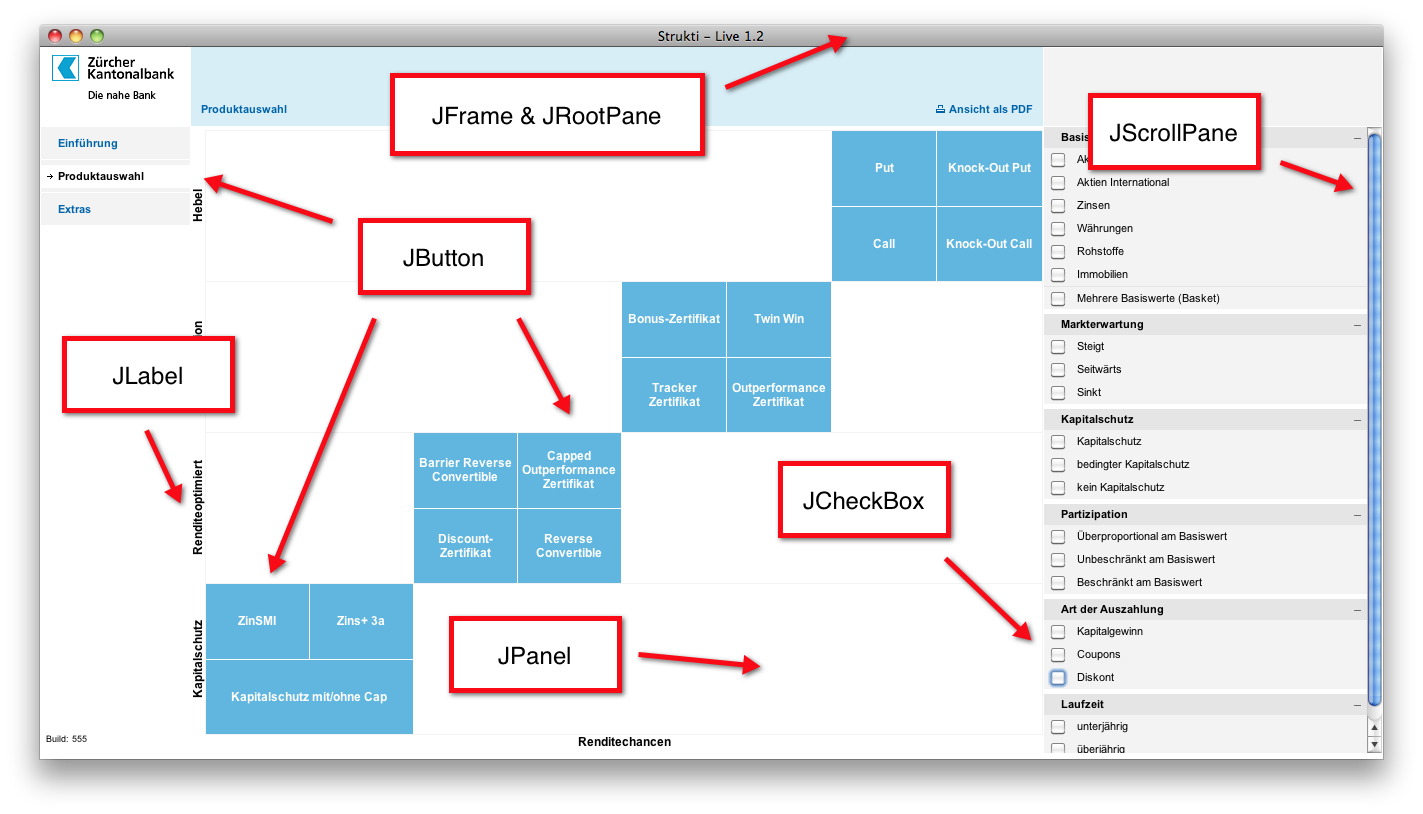
\includegraphics[width=\textwidth]{./image/SL/SL-01.png}
      \caption{Strukti Live 1.2 - Screenshot I}
      \label{img:SL-01}
    \end{center}
  \end{figure}
  
  \begin{figure}[htb]
    \begin{center}
      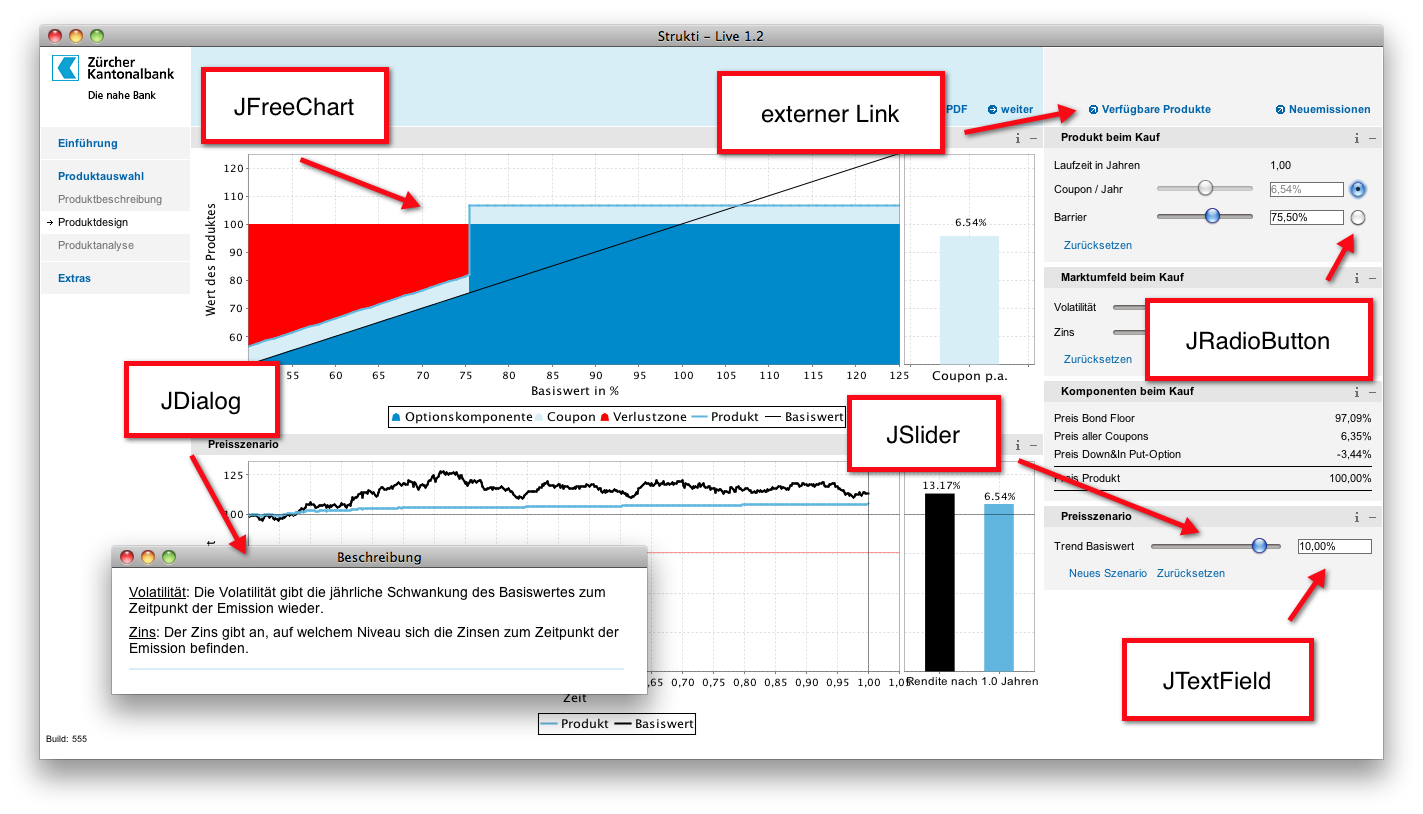
\includegraphics[width=\textwidth]{./image/SL/SL-02.png}
      \caption{Strukti Live 1.2 - Screenshot II}
      \label{img:SL-02}
    \end{center}
  \end{figure}
  
  \begin{figure}[htb]
    \begin{center}
      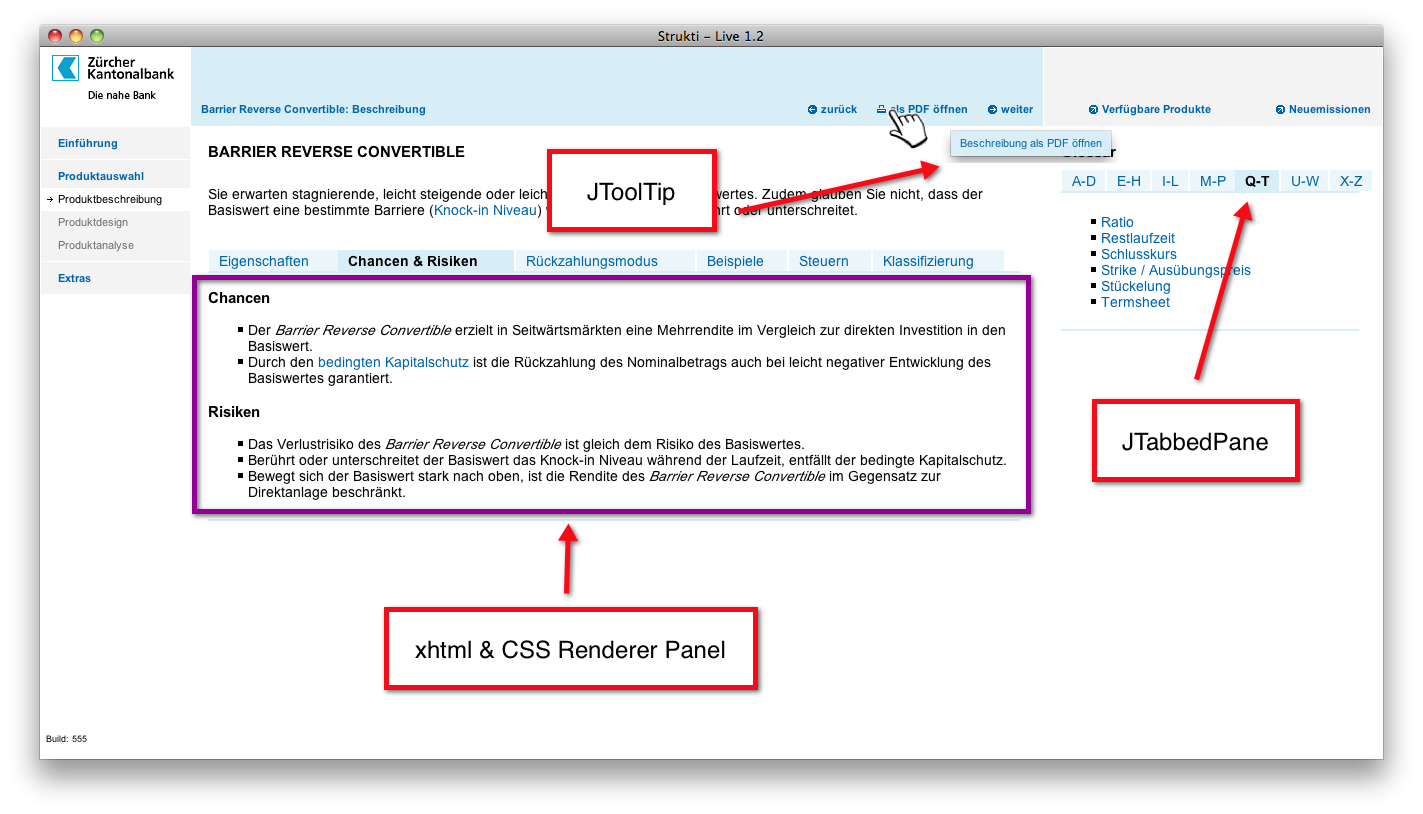
\includegraphics[width=\textwidth]{./image/SL/SL-03.png}
      \caption{Strukti Live 1.2 - Screenshot III}
      \label{img:SL-03}
    \end{center}
  \end{figure}
  
  \subsection{Gefundene Design-Patterns}
  
  \begin{description}
    \item[Observer]
    Die Menüführung wurde durch das Observer-Pattern\footnote{Siehe
    \cite{GUIDesignPatterns} S. 2ff} implementiert. Dabei wird in einem
    Modell durch das Drücken eines \(javax.swing.JButton\) der jeweilige Status
    der Applikation angepasst. Die entsprechen \(javax.swing.JPanel\), welche
    auf Änderungen des Modells hören, können sich dann jeweils neu
    zeichnen.

    Ebenfalls mit dem Observer-Pattern realisiert wurde die Aktualisierung
    von Komponenten welche zusammen hängen. Als Beispiel dient ein Verbund der
    Komponenten \(javax.swing.JTextField\), \(javax.swing.JSlider\) und für die
    grafische Darstellung \(org.jfree.chart.JFreeChart\). Dabei werden bei
    einer Änderung des Wert bei dem \(JSlider\) oder dem \(JTextfeld\) die Werte
    aller anderen Komponenten entsprechend aktualisiert.
  \end{description}
  
  \subsection{Gefundene ``neue'' Komponenten}
  
  \begin{description}
    \item[Button-Matrix]
    \(JButtons\) werden in einer Matrix angeordnet, um sie entsprechend ihrer
    Funktion zu ordnen. Hinter jedem \(JButton\) steckt ein Finanzprodukt, das
    bei einem Klick angezeigt werden kann. Die \(JButtons\) können entsprechend
    ihrer Renditechancen (x-Achse) und deren Kapitalschutzes (y-Achse)
    angeordnet werden.
    \item[Akkordeon]
    Ein Verbund von \(javax.swing.JPanel\) Komponenten, bei welchem ein
    \(JPanel\) als Titelleiste funktioniert. In der Titelleiste kann über ein
    Minus- oder Plussymbol ein weiterer \(JPanel\) ein- oder ausgeklappt werden.
    Zudem gibt es in der Titelleiste ein \(JButton\), wo ein Dialog mit
    Hintergrundinformationen geöffnet werden kann.
  \end{description}
  
  \section{Strukti Online}
  
  Strukti Online ist ein Emissionstool der \ac{ZKB} für strukturierte Produkte.
  Die Applikation wird aktuell nur für den internen Gebrauch entwickelt und
  basiert auf Java Swing. Es wurde die aktuelle Version 2.10.0 für die Analyse
  verwendet.
  
  Da es sich um eine interne Applikation handelt, werden keine Screenshots
  der Applikation gezeigt, da anhand dessen eventuell Rückschlüsse auf die
  Business-Logik gemacht werden könnte.
  
  In der Tabelle \ref{tab:bibliothekenStruktiOnline} sind alle verwendeten
  Bibliotheken, welche eine Interaktion mit dem \ac{GUI} haben, ersichtlich,
  und ob deren Sourcecode zugänglich ist.
  
  \begin{table}[ht]
    \sffamily 
    \begin{center}
      \begin{threeparttable}
        \begin{tabular}{lp{4.5cm}ccp{2cm}}
          \toprule
          \textbf{Bibliothek} & \textbf{Funktion} & \textbf{Version} &
          \textbf{Lizenz} & \textbf{Quellcode vorhanden}\\
          \midrule
          core-renderer.jar & XHtml und CSS Renderer für Swing & R8 & LGPL &
          Ja\\
          jfreechart-1.0.10.jar & Charting Library für Java & 1.0.10 & LGPL
          & Ja\\
          forms.jar & Layout System aus der JGoodies Palette & 1.2.1 &
          BSD\tnote{1} & Ja\\
          swingx-1.0.jar & Swing Komponenten Erweiterung & 1.0 & LGPL & Ja\\
          \bottomrule
        \end{tabular}
        \caption{Verwendete Bibliotheken von Strukti Online 2.10.0}
        \label{tab:bibliothekenStruktiOnline}
        \begin{tablenotes}[++]\footnotesize 
          \item[1] Es handelt sich dabei um die ``BSD open source license''
        \end{tablenotes} 
      \end{threeparttable}
    \end{center}
  \end{table}
  
  \subsection{Gefundene Komponenten}
  
  \subsubsection{Top-Level-Komponenten}
  
  \begin{itemize}
    \item \(javax.swing.JDialog\)
    \item \(javax.swing.JFrame\)
  \end{itemize}
  
  \subsubsection{Intermediate-Komponenten}
  
  \begin{itemize}
    \item \(javax.swing.JLayerdPane\)
    \item \(javax.swing.JPanel\)
    \item \(javax.swing.JRootPane\)
    \item \(javax.swing.JScrollPane\)
    \item \(javax.swing.JTabbedPane\)
  \end{itemize}
  
  \subsubsection{Atomic-Komponenten}
  \begin{itemize}
    \item \(javax.swing.JButton\)
    \item \(javax.swing.JCheckbox\)
    \item \(javax.swing.JComboBox\)
    \item \(javax.swing.JFileChooser\)
    \item \(javax.swing.JLabel\)
    \item \(javax.swing.JRadioButton\)
    \item \(javax.swing.JPasswordField\)
    \item \(javax.swing.JSeparator\)
    \item \(javax.swing.JSlider\)
    \item \(javax.swing.JSpinner\)
    \item \(javax.swing.JTable\)
    \item \(javax.swing.JTextArea\)
    \item \(javax.swing.JTextField\)
    \item \(javax.swing.JTextPane\)
    \item \(javax.swing.JToolTip\)
  \end{itemize}
  
  \subsubsection{Spezielle Komponenten}
    
  \begin{itemize}
    \item \(javax.swing.JLabel\) als externer Link
    \item \(org.jfree.chart.JFreeChart\)
    \item \(org.xhtmlrenderer.simple.XHTMLPanel\)
    \item \(org.jdesktop.swingx.JXBusyLabel\)
    \item \(org.jdesktop.swingx.JXDatePicker\)
  \end{itemize}
    
  \subsection{Gefundene Design-Patterns}
  
  \begin{description}
    \item[MVC]
    Das Zusammenspiel von Model, View und Kontroller wurde strikte nach dem
    MVC Design-Pattern\footnote{Siehe \cite{GUIDesignPatterns} S. 15ff.}
    implementiert.
    
    \item[Observer]
    Einfache Aktualisierungen zwischen Komponenten wurden strikte nach dem
    Observer Design-Pattern\footnote{Siehe \cite{GUIDesignPatterns} S. 2ff.}
    implementiert.
    
    \item[Tabellen-Filter]
    Durch die Verwendung von \(JRadioButton\), \(JComboBox\), \(JXDatePicker\)
    und \(JSpinner\) wurden, bei den meisten Ansicht von Tabellen, Filter gebaut,
    damit die Daten auf das Wesentliche reduziert werden können. Datei wurde
    für jede relevante Spalten der Tabelle, entsprechend deren Datentyp, eine
    dieser Komponenten gewählt.
  \end{description}
  
  \subsection{Gefundene ``neue'' Komponenten}
  
  \begin{description}
    \item[Button-Matrix]
    \(JButtons\) werden in einer Matrix angeordnet, um sie entsprechend ihrer
    Funktion zu ordnen. Hinter jedem \(JButton\) steckt ein spezifisches
    vorbewertetes Finanzprodukt, das bei einem Mouseklick angezeigt werden
    kann. Die \(JButtons\) können entsprechend ihrer Laufzeit (x-Achse) und der
    Underlyings\footnote{Auch Basiswerte genannt, siehe \cite{Basiswerte}} des
    hinterlegten Finanzprodukts (y-Achse) angeordnet werden. Die Matrix, kann
    wie eine Tabelle nach Laufzeiten sortiert werden.
    
    \item[Akkordeon]
    Ein Verbund von \(javax.swing.JPanel\) Komponenten, bei welchem ein
    \(JPanel\) als Titelleiste funktioniert. In der Titelleiste kann über ein
    Minus- oder Plussymbol ein weiterer \(JPanel\) ein- oder ausgeklappt werden.
    
    \item[Zeit-Panel]
    Durch die Kombination einer \(org.jdesktop.swingx.JXDatePicker\) und einer
    \(javax.swing.JSpinner\) Komponente kann ein Datum mit Uhrzeit ausgewählt
    werden.
  \end{description}
  
  \section{Hedo Tool}
  
  Hedo Tool ist eine Applikation zur Gewichtung verschiedener Rating-Modelle
  für Wohneigentum. Die Applikation wird aktuell nur zum internen Gebrauch
  entwickelt und basiert auf Java Swing. Es wird die aktuelle Version 1.0.710
  für die Analyse verwendet.
  
  Da es sich um eine interne Applikation handelt, werden keine Screenshots der
  Applikation gezeigt, da anhand dessen eventuell Rückschlüsse auf die
  Business-Logik gemacht werden könnte.
  
  In der Tabelle \ref{tab:bibliothekenHedoTool} sind alle verwendeten
  Bibliotheken, welche eine Interaktion mit dem \ac{GUI} haben, ersichtlich,
  und ob deren Sourcecode zugänglich ist.
  \newline
  
  \begin{table}[ht]
    \sffamily 
    \begin{center}
      \begin{threeparttable}
        \begin{tabular}{lp{4.5cm}ccp{2cm}}
          \toprule
          \textbf{Bibliothek} & \textbf{Funktion} & \textbf{Version} &
          \textbf{Lizenz} & \textbf{Quellcode vorhanden}\\
          \midrule
          binding-2.0.6.jar & Swing Data Binding Framework aus der JGoodies
          Palette & 2.0.6 & BSD\tnote{1} & Ja\\
          forms.jar & Layout System aus der JGoodies Palette & 1.2.1 &
          BSD\tnote{1} & Ja\\
          swingx-1.0.jar & Swing Komponenten Erweiterung & 1.0 & LGPL & Ja\\
          validation-2.0.1.jar & Validiert und präsentiert Validationsresultate
          & 2.0.1 & BSD\tnote{1} & Ja\\
          \bottomrule
        \end{tabular}
        \caption{Verwendete Bibliotheken von Hedo Tool 1.0.710}
        \label{tab:bibliothekenHedoTool}
        \begin{tablenotes}[++]\footnotesize 
          \item[1] Es handelt sich dabei um die ``BSD open source license''
        \end{tablenotes} 
      \end{threeparttable}
    \end{center}
  \end{table}
  
  \subsection{Gefundene Komponenten}
  
  \subsubsection{Top-Level-Komponenten}
  
  \begin{itemize}
    \item \(javax.swing.JDialog\)
    \item \(javax.swing.JFrame\)
  \end{itemize}
  
  \subsubsection{Intermediate-Komponenten}
  
  \begin{itemize}
    \item \(javax.swing.JLayerdPane\)
    \item \(javax.swing.JPanel\)
    \item \(javax.swing.JRootPane\)
    \item \(javax.swing.JScrollPane\)
  \end{itemize}
  
  \subsubsection{Atomic-Komponenten}
  
  \begin{itemize}
    \item \(javax.swing.JButton\)
    \item \(javax.swing.JCheckbox\)
    \item \(javax.swing.JComboBox\)
    \item \(javax.swing.JFileChooser\)
    \item \(javax.swing.JFormattedTextField\)
    \item \(javax.swing.JLabel\)
    \item \(javax.swing.JMenuBar\)
    \item \(javax.swing.JMenu\)
    \item \(javax.swing.JMenuItem\)
    \item \(javax.swing.JProgressBar\)
    \item \(javax.swing.JSeparator\)
    \item \(javax.swing.JSpinner\)
    \item \(javax.swing.JTable\)
    \item \(javax.swing.JTextField\)
    \item \(javax.swing.JTextPane\)
    \item \(javax.swing.JToolTip\)
  \end{itemize}
  
  \subsubsection{Spezielle Komponenten}
    
  \begin{itemize}
    \item \(javax.swing.JLabel\) als externer Link
    \item \(org.jdesktop.swingx.JXBusyLabel\)
  \end{itemize}
  
  \subsection{Gefundene Design-Patterns} 
  
  \begin{description}
    \item[MVC]
    Das Zusammenspiel von Model, View und Kontroller wurde strikte nach dem
    MVC Design-Pattern\footnote{Siehe \cite{GUIDesignPatterns} S. 15ff.}
    implementiert.
    
    \item[Observer]
    Einfache Aktualisierungen zwischen Komponenten wurden strikte nach dem
    Observer Design-Pattern\footnote{Siehe \cite{GUIDesignPatterns} S. 2ff.}
    implementiert.
    
    \item[Worker]
    Asynchrone Jobs, die viel Rechenzeit in Anspruch nehmen, wurden mit\\
    \(javax.swing.SwingWorker\) gelöst.
  \end{description}
  
  \subsection{Gefundene ``neue'' Komponenten}
  
  Es wurden keine ``neuen'' Komponenten identifiziert.
  
  \section{Liste der Komponenten}
  
  Die Auflistung aller gefunden Komponenten soll die vereinigte Menge aller
  gefundenen Komponenten widerspiegeln. Die Auflistung soll als Grundlage für
  die Analyse, ob eine Implementierung der erkannten Swingkomponenten möglich
  ist, dienen. Folgende 32 Komponenten wurden in den Applikationen gefunden:
  
  \subsection{Top-Level-Komponenten}
  
  \begin{itemize}
    \item \(javax.swing.JDialog\)
    \item \(javax.swing.JFrame\)
  \end{itemize}
  
  \subsection{Intermediate-Komponenten}
  
  \begin{itemize}
    \item \(javax.swing.JLayerdPane\)
    \item \(javax.swing.JPanel\)
    \item \(javax.swing.JRootPane\)
    \item \(javax.swing.JScrollPane\)
    \item \(javax.swing.JTabbedPane\)
  \end{itemize}
  
  \subsection{Atomic-Komponenten}
  
  \begin{itemize}
    \item \(javax.swing.JButton\)
    \item \(javax.swing.JCheckbox\)
    \item \(javax.swing.JComboBox\)
    \item \(javax.swing.JFileChooser\)
    \item \(javax.swing.JFormattedTextField\)
    \item \(javax.swing.JLabel\)
    \item \(javax.swing.JMenuBar\)
    \item \(javax.swing.JMenu\)
    \item \(javax.swing.JMenuItem\)
    \item \(javax.swing.JPasswordField\)
    \item \(javax.swing.JProgressBar\)
    \item \(javax.swing.JRadioButton\)
    \item \(javax.swing.JSeparator\)
    \item \(javax.swing.JSlider\)
    \item \(javax.swing.JSpinner\)
    \item \(javax.swing.JTable\)
    \item \(javax.swing.JTextArea\)
    \item \(javax.swing.JTextField\)
    \item \(javax.swing.JTextPane\)
    \item \(javax.swing.JToolTip\)
  \end{itemize}
  
  \subsection{Spezielle Komponenten}
  
  \begin{itemize}
    \item \(javax.swing.JLabel\) als externer Link
    \item \(org.jfree.chart.JFreeChart\)
    \item \(org.xhtmlrenderer.simple.XHTMLPanel\)
    \item \(org.jdesktop.swingx.JXBusyLabel\)
    \item \(org.jdesktop.swingx.JXDatePicker\)
  \end{itemize}
  
  \section{Liste der GUI Paradigmen}
  
  Die Auflistung aller gefundenen GUI Paradigmen soll die vereinigte Menge aller
  gefundenen GUI Paradigmen widerspiegeln. Die Auflistung soll als Grundlage für
  die Analyse, ob eine Implementierung der erkannten GUI Paradigmen möglich
  ist, dienen. Folgende sieben GUI Paradigmen wurden in den Applikationen
  gefunden:
      
  \subsection{Design-Patterns}
  
  \begin{itemize}
    \item MVC
    \item Observer
    \item Tabellen-Filter
    \item Worker
  \end{itemize}
  
  \subsection{``Neue'' Komponenten}
  
  \begin{itemize}
    \item Button-Matrix
    \item Akkordeon
    \item Zeit-Panel
  \end{itemize}